\documentclass{jsarticle}
\usepackage[dvipdfmx]{graphicx}

\title{楽しい運動計測実習に関するレポート}
\date{\today}
\author{奥屋 直己}

\usepackage[height=26cm,width=16cm]{geometry}

\graphicspath{{./images/}}

\begin{document}

\maketitle

\section{実験の目的}

人間の腕はどうして同じ速さで運動し続けることができるのだろうか。例えば、車や自転車に乗っているとき、アクセルのみで同じ速さを保とうとしても難しい。どうしても早くなってしまう。だが、ブレーキを使うと同じ速さを保ち続けるのは容易である。このことから、人間の腕にもブレーキが存在しているのではないかと考える。本レポートでは、腕を伸ばす、曲げるの繰り返し運動を行うことで、ブレーキが存在するかどうかを確かめた。

\section{手法}

\subsection{実験}

本実験は2人の被験者に右腕を水平面内で伸ばす、曲げるの繰り返し運動を楽と思える速さで動かす場合とそれよりも速く動かす場合の2種類を行うよう指示した。ただし、1人のデータをうまく取ることが出きなかったため、実質データは1人分となった。運動中の手首、肘、肩の3点に反射マーカーをつけ、高速度カメラを使い、それぞれの軌道を計測した。筋電位は、上腕二頭筋と上腕三頭筋に筋電計用電極を取り付け計測した。それぞれ、サンプリング周波数は軌道を1000 [fps]、筋電位を200 [Hz]とし、同時パルス発生装置を使い、開始時刻を同期した上で20秒間計測した。
\subsection{解析}

今回は筋電センサ(LOGICAL PRODUCT:ワイヤレス筋電センサ乾式)による筋電データとモーションキャプチャ(Library:Move-tr/3D)による運動軌道データを別々のプログラムで作成する。

\subsubsection{筋電データ}

筋電データにデータの1〜40Hzに対してバンドパスフィルタ(3次バターワークス)をかけた。また、それによって起きる時間的なズレを修正するため、順方向と逆方向の両方から1回ずつフィルタをかけ、ズレをなくした。

次に筋肉の活動度a(t)を以下の式で評価した。

\begin{equation}
a(t)=\frac{1}{\Delta{T}}\int^{t+\Delta{T}/2}_{t-\Delta{T}/2} |E(t)|dt
\end{equation}

E(t)は筋電位、tは時間、幅$\Delta{T}$の窓を0.2 [t]とした。

\section{結果}

図\ref{fig:motion1}が楽な速さでの腕の軌道、図\ref{fig:motion2}が速く動かす時の腕の軌道である。この2つの図を比較すると、軌道に大きな差がないことがわかる。図\ref{fig:EMG1}を見ると、上腕二頭筋の筋電位のピーク位置と、上腕三頭筋の筋電位のピーク位置がほぼ同じ時間にあることがわかる。図\ref{fig:+length}をみると腕を曲げる時に筋電位のピーク位置がある。腕を曲げるために上腕二頭筋、伸ばすために上腕三頭筋を使うことから、腕を曲げるときに上腕三頭筋が上腕二頭筋の運動を阻害していることがわかった。図\ref{fig:EMG2}を見ると、上腕二頭筋が筋電位のピーク位置のときと、上腕三頭筋のピーク位置の位相が反対になっており、速く動かすときは上腕二頭筋と上腕三頭筋がそれぞれの運動を阻害していない。これらより、運動の速さによって上腕三頭筋の使われ方が違うことがわかった。
\begin{figure}[htbp]
  \begin{minipage}{0.5\hsize}
    \begin{center}
      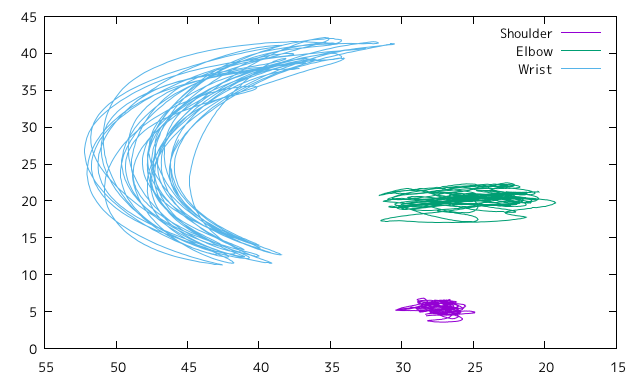
\includegraphics[clip,width=80mm]{Graph_2.png}
      \caption{指示していない速さでの運動での手首、肘、肩の3点の軌道(青=手首の軌道,緑=肘の軌道,紫=肩の軌道)。肘と肩はほぼ一定の位置で手首の軌道のみ大きく動いており、指示通りに腕を動かせていることがわかる。\label{fig:motion1}}
    \end{center}
  \end{minipage}
  \begin{minipage}{0.5\hsize}
    \begin{center}
      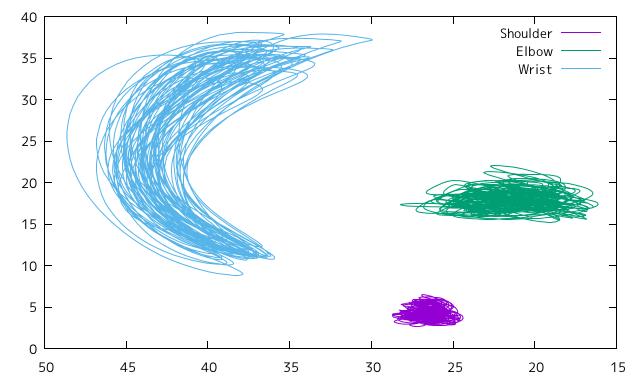
\includegraphics[clip,width=80mm]{Graph_3.png}
      \caption{図\ref{fig:motion1}よりも速く動かすように指示した場合の手首、肘、肩の3点の軌道(青=手首の軌道,緑=肘の軌道,紫=肩の軌道)。 図\ref{fig:motion1}と同様に手首のみが大きく動いており、指示通りに動かせていることがわかる。\label{fig:motion2}}
    \end{center}
  \end{minipage}
\end{figure}

\begin{figure}[htbp]
  \begin{minipage}{0.5\hsize}
    \begin{center}
      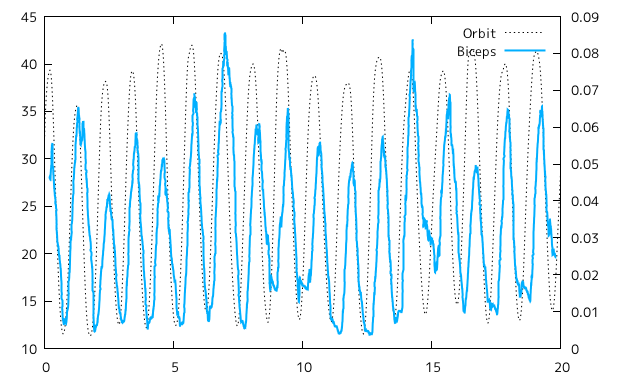
\includegraphics[clip,width=80mm]{Graph_4.png}
      \caption{指示していない速さで運動した時の上腕二頭筋と上腕三頭筋の筋電位(上腕二頭筋=青,上腕三頭筋=緑)。どちらの筋電にも腕の運動に合わせて振動している。 \label{fig:EMG1}}
    \end{center}
  \end{minipage}
  \begin{minipage}{0.5\hsize}
    \begin{center}
      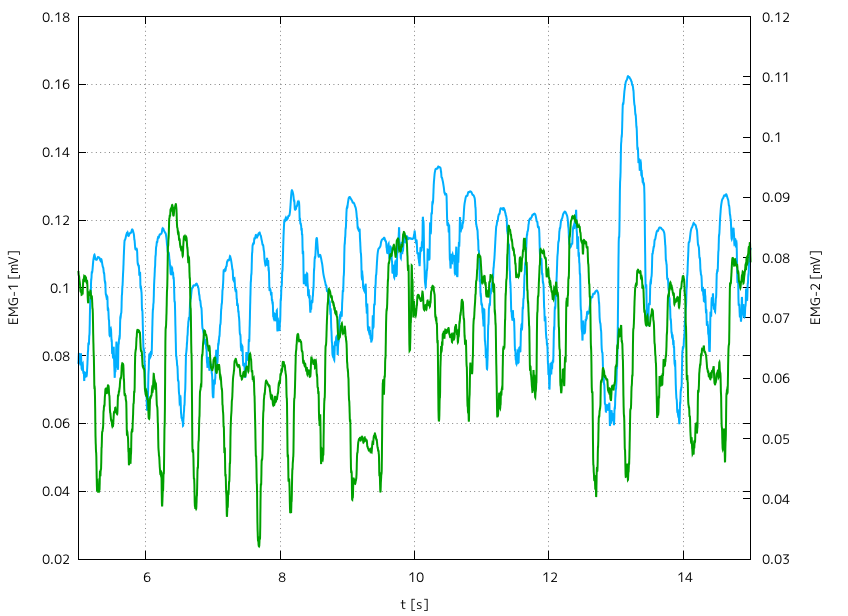
\includegraphics[clip,width=80mm]{Graph_5.png}
      \caption{速く動かす運動をした時の上腕二頭筋と上腕三頭筋の筋電位(上腕二頭筋=青,上腕三頭筋=緑)。左側のY軸が上腕二頭筋、右側のY軸が上腕三頭筋の筋電位を表す。 どちらの筋電にも腕の運動に合わせて振動している。\label{fig:EMG2}}
    \end{center}
  \end{minipage}
\end{figure}

\begin{figure}[htbp]
  \begin{center}
    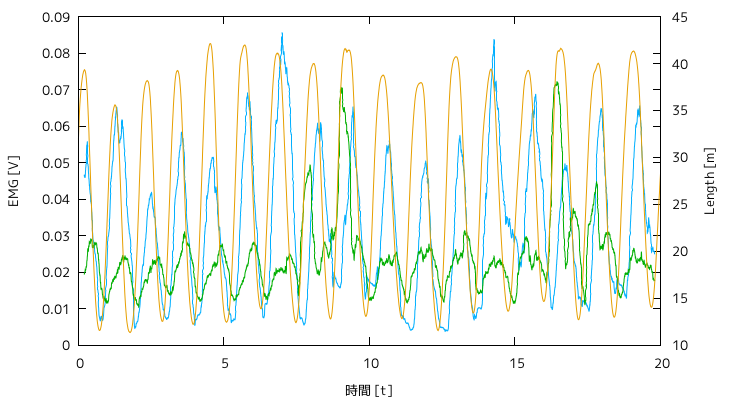
\includegraphics[clip,width=80mm]{Graph_6.png}
    \caption{図\ref{fig:EMG1}に図\ref{fig:motion1}から手首の運動軌道のY軸を重ねた図。左Y軸が筋電位(上腕二頭筋=青,上腕三頭筋=緑)、右Y軸が手首の移動距離(=黄色)となっている。手首の軌道はピーク位置の時、腕は伸びている。\label{fig:+length}}
  \end{center}
\end{figure}

  
\section{考察}
結果より、楽な速さの時、腕を曲げるとき、上腕三頭筋は上腕二頭筋を阻害するように力が働く。逆に速く動かすとき、上腕三頭筋は阻害しないように運動する。このことから、楽な速さで動かす場合に上腕三頭筋がブレーキの役割を担い、速さを一定に保っているのではないかと考える。また、速く動かしたときは、上腕三頭筋がブレーキをかけないことによって、速く動かすことができるのではないかと考える。今実験では行わなかったが、楽に動かす速さよりも遅く動かした場合、上腕三頭筋の筋電位が大きく反応するのではないかと考える。
\end{document}